\npchapter{Reference Architecture}
As mentioned in the introduction, this work is written in cooperation with SAP.\par
In fact, the limitations mentioned in the previous chapter are deducted from the limitations the SAP Gardener team struggles with themselves. Therefore, this chapter introduces the \textit{Open Component Model (OCM)}, SAP Gardener's proposed standard to automate software delivery and decouple the compliance scans from the CI/CD pipeline.\par
Thereon, the abstract design for the \emph{Security and Compliance Data Lake} is developed. This abstract design is then used to derive an entire holistic solution architecture for modern development and deployment landscapes to overcome the limitations of the current state of the art approach.

\section{Open Component Model} \label{sec:Open Component Model}
The OCM is a SBOM format created and used by SAP Gardener. It does not fulfill the minimum requirements as defined by the NTIA. But this is due to the fact that the OCM has a different focus than SPDX or CycloneDX. While those two were deliberately designed to be a bill of materials, thoroughly listing the decomposition of a software, the OCM was specifically developed to decouple CI from CD and thereby overcome related limitations such as the ones mentioned in the previous chapter.\par 
So, SPDX effectively describes \emph{arbitrary metadata} (e.g. licenses and file type) about logical units of software. SPDX refers to this logical units of software as \emph{Packages}. As described in section \ref{sec:SBOM} "Software Bill of Materials", a \emph{Package} may be anything, ranging from a snippet of code over single file over an artifact to an entire software product version. Thus, SBOMs are \emph{containers for arbitrary software metadata}.\par
Opposed to that, the OCM describes the \emph{delivery relevant information about and the access to artifacts} composing a logical unit of software. OCM refers to this logical units of software as \emph{Components}, or rather \emph{Component Versions}. Thus, \emph{Component Versions} are  \emph{containers for a structured set of delivery relevant artifacts}.\par 
For this reason, SAP Gardener stopped referring to OCM as an SBOM format and instead invented the term \emph{Software Bill of Delivery (SBOD)}.\par
Following is a technical explanation of the OCM deducted from the specification \cite{OCMSpec}, an internal presentation \cite{OCMInternalPresentation} and interviews with responsible developers. Even though this explanation focuses on understanding the rationale behind the design decisions of the proposed standard rather than technical completeness, it may still be hard to grasp. This is due to the abstract nature of the OCM. Therefore, emphasis and examples are used where possible. Also, while the textual description explains the OCM as the abstract model that it is, figure \ref{fig:ComponentDescriptor} below shows a \emph{Component Descriptor}, the serialization format of a \emph{Component Version}. This may also support in understanding the abstract concepts.

\subsection{Model Elements}

\noindent\textbf{Component}\\
"A \emph{Component} is an abstract entity describing a dedicated usage context or meaning for provided software. It is technically defined by a \emph{globally unique identifier}"\cite{OCMSpec} (l. 2). With this globally unique identifier, a \emph{Component} acts as a namespace for multiple \emph{Component Versions}. So the \emph{Component} identified by the name \lstinline|github.com/gardener/etcd-druid| contains software versions of a product, a druid, that helps configuring \emph{etcd}, a central key-value store, in Kubernetes clusters deployed by SAP Gardener.\\

\noindent\textbf{Component Version}\\
As already described, a \emph{Component Version} describes a structured set of concrete \emph{Artifacts}. It is technically defined by the globally unique identifier of the \emph{Component} and a version (ll. 2-3). Thus, a \emph{Component Version} is an instance of a \emph{Component} adhering to the semantic, thus, the usage context or meaning, given by the name. A \emph{Component Version} leverages essentially two mechanisms to describe this structured set of \emph{Artifacts}. 
\begin{enumerate}
\item A \emph{Component Version} may describe the delivery relevant information about and the access to an artifact directly (ll. 9-22, ll. 23-39).
\item A \emph{Component Version} may describe a reference to another \emph{Component Version} to include its described set of artifacts indirectly (ll. 40-56).
\end{enumerate}

\noindent\textbf{Artifacts and Component References}\\
The two model elements enabling those artifact composing mechanisms are \emph{Artifacts} (ll. 9-22, ll. 23-39) and \emph{Component References} (ll. 40-56). Thereby, drawing an analogy to file systems, \emph{Artifacts} and their identities correspond to files and their names and \emph{Component References} and their identities are analogous to directories and their names. Thus, \emph{Component References} also impose a structure on the artifact set, like a directory tree that provides access to a structured set of named data content (the files).\par
\noindent Both those model elements share common sets of attributes \cite{OCMSpec}:\\

\textbf{Identity:} The \emph{Identity} attribute set composes a \emph{Component Version-Local Identity}. Thus, it uniquely identifies the elements in the context of a \emph{Component Version}. The \emph{Identity} at least consists of a \emph{name}.\par 
The \lstinline|name| \emph{(string)}  (l. 10, l. 24, l. 41) is \emph{required} and should be chosen to be unique within the \emph{Component Version}. But it also carries semantic information, the meaning or purpose of the element. So, a \emph{Component Version} may describe a REST application. This REST application may use a nginx version as HTTP server and a different nginx version as load balancer. In order to have the flexibility to name them both "nginx" the \emph{Identity} has two additional optional attributes, \emph{version} and \emph{extra identity}.\par
The \lstinline|version| \emph{(string)} (l. 16, l. 25, l. 43) is \emph{optional} and describes the version of the respective model elements.\par
The \lstinline|extraIdentity| \emph{(map[string]string)}(l. 17, l. 32, ll. 45-46) is \emph{optional} and allows adding arbitrary identity attributes.\par
As this is a \emph{Component-Version-Local Identity}, \emph{Artifacts} and \emph{Component References} may be identified by the triple \emph{({Component Name}, {Component Version}, {Local Identity})}.\\

\textbf{Labels:} The \emph{Labels} attribute set is represented by a single \lstinline|labels| \emph{([]any)} attribute. With this, \emph{Labels} allows to attach additional arbitrarily nested metadata to such an element, which is not directly described by the existing model elements. This enables the use of application specific attributes without the need to extend the model for new arising use cases \cite{OCMSpec}. When a \emph{Component Version} is used by a tool to retrieve the artifacts of the respective product version and put them into a scanning tool, a tag within the labels attribute could be used to mark exceptions, e.g. an artifact within that product version that does never have to be scanned.
\begin{figure}[H]
\begin{minted}[
frame=single,
fontsize=\tiny,
linenos,
numbersep=-10pt,
obeytabs=true
]{YAML}
    component:
      name: github.com/gardener/etcd-druid
      version: v0.15.3
      repositoryContexts:
        - type: ociRegistry
          baseUrl: eu.gcr.io/sap-se-gcr-k8s-private/cnudie/gardener/development
          subPath: null
      provider: internal
      sources:
        - name: github_com_gardener_etcd-druid
          access:
            type: github
            repoUrl: github.com/gardener/etcd-druid
            ref: refs/tags/v0.15.3
            commit: a6112534eb79021fa191edb8efd6512760ae050f
          version: v0.15.3
          extraIdentity: {}
          type: git
          labels:
            - name: cloud.gardener/cicd/source
              value:
                repository-classification: main
      resources:
        - name: etcd-druid
          version: v0.15.3
          type: ociImage
          access:
            type: ociRegistry
            imageReference: >-
              eu.gcr.io/sap-se-gcr-k8s-public/eu_gcr_io/gardener-project/gardener/etcd-druid:v0.15.3-mod1
          digest: null
          extraIdentity: {}
          relation: local
          labels:
            - name: cloud.gardener.cnudie/migration/original_ref
              value: eu.gcr.io/gardener-project/gardener/etcd-druid:v0.15.3
            - name: cloud.gardener.cnudie/sdo/lssd
              value:
                processingRules:
                  - purge_berkeleydb_to_public
          srcRefs: []
      componentReferences:
        - name: etcd
          componentName: github.com/gardener/etcd-custom-image
          version: v3.4.13-bootstrap-8
          digest: null
          extraIdentity:
            imagevector-gardener-cloud+tag: v3.4.13-bootstrap-8
          labels:
            - name: imagevector.gardener.cloud/images
              value:
                images:
                  - name: etcd
                    repository: eu.gcr.io/gardener-project/gardener/etcd
                    resourceId:
                      name: etcd
                    sourceRepository: github.com/gardener/etcd-custom-image
                    tag: v3.4.13-bootstrap-8
      labels: []
    signatures: []
\end{minted}
	\centering
	\caption[Component Descriptor]{Component Descriptor \source{Based on \cite{OCMSpec}}}
	\label{fig:ComponentDescriptor}
\end{figure}

\noindent\textbf{Artifacts}\\
Generally, an \emph{Artifact} is a blob containing some data in some technical format \cite{OCMSpec}. Besides \emph{Identity} and \emph{Labels}, \emph{Artifacts} do have the following further attributes \cite{OCMSpec}:
\begin{itemize}
\item A dedicated globally unique \lstinline|type| (l. 18, l. 26) representing the kind of content and how it can be used.
\item A formal description of the \lstinline|access| (ll. 11-15, ll. 27-30). This description can be used to technically access the content of the artifact in form of a blob with a format defined by the \lstinline|type| of the artifact (l. 18, l. 26) (the \lstinline|type| shown within the access in figure \ref{fig:ComponentDescriptor} specifies the access method and thereby determines the fields of the access specification).
\end{itemize}
The OCM distinguishes two kinds of \emph{Artifacts}, \emph{Sources} and \emph{Resources}.\par
\emph{Sources} (ll. 9-22) describe artifacts that are sources for the delivery relevant artifacts (e.g. source code).\par
\emph{Resources} (ll. 23-41) describe delivery artifacts, intended for deployment into a runtime environment (e.g. executables or OCI Images) or additional content relevant for deployment mechanisms (e.g. helm charts). Thus, these are the artifacts built from \emph{Sources}. The connection may be expressed through the \lstinline|srcRef| attribute which is an additional attribute only existing for \emph{Resources} \cite{OCMSpec}.\\

\noindent\textbf{Component References}\\
A \emph{Component Version} may refer to other \emph{Component Versions} by adding a \emph{Component Reference} (ll. 42-58). As already mentioned, through this mechanism, the referring \emph{Component Version} includes the artifact set described by the referred \emph{Component Version}.\par
Important to stress here is, that \emph{Component References} do not only specify the \emph{Identity} of the referenced \emph{Component Version} but do also have the \emph{Component Version-Local Identity}. Thus, the reference itself has an \emph{Identity} within the \emph{Component Version} just like \emph{Artifacts}. Since the name of this \emph{Local Identity} carries the semantic information about the meaning or purpose of the identified piece of software in the context of the \emph{Component Version}, this allows referencing the same \emph{Component Version} twice with different meaning. This purpose can then be used by tools evaluating a \emph{Component Version} to find the correct \emph{Artifact} or \emph{Component Reference} for the specific use case. Therefore, local identities should be kept stable among successive versions of a \emph{Component}.\par
But since the referenced \emph{Component Version} still has to be specified, the \emph{Component Reference} has an additional attribute, \lstinline|componentName| (l. 44), which, together with \lstinline|version| (l. 45), uniquely identifies the \emph{Component Version} \cite{OCMSpec}.\\

\noindent\textbf{Additional Information}\\
There are some attributes in figure \ref{fig:ComponentDescriptor} that are less important, but shall still be mentioned for completeness of the description \cite{OCMSpec}:
\begin{itemize}
\item A \emph{Repository Context} (ll. 4-7) describes the access to an \emph{OCM Repository}. An \emph{OCM Repository} thereby is a repository providing technical access to the \emph{Component Version}, or rather the \emph{Component Descriptor}. 
\item The \emph{Provider} (l. 8) specifies the company or organization providing the \emph{Component Version}.
\item A \emph{Component Version} may have \emph{Labels} (l. 59) itself, to attach additional information. 
\item A \emph{Component Version} may be signed by some authority to ensure that it can be trusted. The \emph{signatures} (ll. 60) attribute may contain multiple signatures, where each entry specifies a name for the signature, the digest value for the signature alongside its respective hash- and normalization algorithm and the signature itself. The digest of the \emph{Component Version} thereby includes the digests of the delivery relevant artifacts, thus, the \emph{Resources}, which may be stored alongside their respective descriptions (l. 31).
\end{itemize}

For further or more detailed information about specific elements or the Open Component Model and its ecosystem in general, refer to the official documentation \cite{OCMSpec}.

\subsection{Capabilities of the Open Component Model}
After the abstract description, this brief section revisions the major concepts of and points out the most important capabilities enabled by the \emph{Open Component Model}.\\

\noindent\textbf{Aggregation Mechanism}\\
\emph{Components} and \emph{Component Versions} respectively are an abstract concept, defined in a way that allows to describe the artifact set and its delivery relevant information for arbitrary aggregations ranging from a specific \emph{software product} over \emph{artificial aggregations} like all artifacts used by the SAP Gardener CI/CD team to an entire \emph{application landscape}.\par
So, a \emph{Component Version} named "SAP Gardener CI/CD" could have \emph{Component References} to all \emph{Component Versions} describing a software product used within the SAP Gardener CI/CD team. The \emph{Component Version} hierarchy created through these \emph{Component References} would thereby indirectly specify their complete set of \emph{Artifacts}.\\

\noindent\textbf{Access Automation}\\
As each of these \emph{Artifacts} describes the access to the technical artifact in a machine-readable format, a tool may automatically find all the relevant technical artifacts and deploy them into a specific environment or provide them to scanning tools.\par
With that, the Open Component Model enables a \emph{holistic deployment automation} and a \emph{decoupling of compliance scans from the CI/CD pipeline} based on \emph{Component Versions}.\\ 

\noindent\textbf{Technology-Agnostic and Access-Independent Identification Scheme}\\
The OCM introduces a \emph{technology-agnostic identification scheme} based on the component namespace. Thus, an artifact is addressed through its semantic within the \emph{Component} independent of its technology - to be concrete the triple \emph{({Component Name}, {Component Version}, {Local Artifact Identity})}.\par
A \emph{Component Version} might describe a software product. This software product includes a Java library as an \emph{Artifact} with a \emph{Local Artifact Identity}, e.g. "JavaLib". This Java library may be stored in a Maven repository where it is identified by its group id (uniquely identifies a project across all maven projects), artifact id (uniquely identifies a artifact within a project) and version (e.g. org.example:javalib:1.0.0). Additionally, it may be stored in a local artifact repository where it is identified by a digest of its contents.\par
To switch the location where the artifact will be accessed by tools evaluating the \emph{Component Version} describing the artifact, only the \emph{access} has to be exchanged without affecting the identity through which the \emph{Artifact} is addressed.\par 
This is also important in complex development and deployment landscapes as it provides additional flexibility. Due to national restrictions, one might be obligated to deploy artifacts from artifact repositories located in the respective country. Hence, different \emph{Component Repositories} may store \emph{Component Descriptors} for a specific \emph{Component Version} with different \emph{access} properties. Thus, the \emph{access} properties may be exchanged transparently without affecting the deployment automation.\par
As \emph{Component Versions}, or rather their serialization format \emph{Component Descriptors}, are also stored in repositories, the statement in section \ref{sec:Integrating Security and Compliance Measures} "Integrating Security and Compliance Measures", that it is convenient to feed respective tools from repositories, still fits.\par
But opposed to this, \emph{the OCM is technology-agnostic and thereby forms a transparency layer, linking different storage locations and content technologies (e.g. artifact repositories or source repositories) and tools (e.g. scanning tools)}.\\

To conclude this, the Open Component Model solves several limitation of the state of the art approach. It provides an \emph{aggregation for artifacts and thereby bridges the gap between a specific software installation to the therein used artifacts}. With this, it also introduces a \emph{uniform identification and access scheme} for these artifacts, making them conveniently accessible for SCA tools independent of their technology or CI/CD pipeline.\par
The data lake still has to use this structural information about the artifact composition of software products and connect it to the information about contained packages and further metadata (e.g. vulnerabilities or licenses) provided by arbitrary data sources (e.g. scanning tools or build tools) with different individual identification schemes. 

\section{Abstract Solution Idea}
The \emph{Open Component Model} with its abstract properties, or rather capabilities, explained in the previous section, builds the foundation for the \emph{Security and Compliance Data Lake}. Thereby, the \emph{Open Component Model} could also be replaced by other standard providing similar capabilities. From hereon, such standards are generally referred to as \emph{Component Models} for the further context of the thesis.\par
Based on such a \emph{Component Model}, this section deducts and outlines an abstract data lake design. Building upon this, it describes a \emph{reference architecture} for integrating the \emph{Data Lake} into a modern development and deployment landscape and a \emph{holistic solution architecture} to overcome all the limitations of the state of the art approach.

\subsection{Abstract Data Lake Design}
Figure \ref{fig:AbstractDataLakeDesign} outlines the abstract data lake design based on a \emph{Component Model}.\\

As shown, the \emph{Component Model} is at the center of the \emph{Data Lake}. The information about \emph{Components} and the therein effectively used artifacts is provided by the \emph{Component Model} directly.\par
Through the access automation, the artifacts may be fed into scanning tools to obtain the  decomposition information about the \emph{Packages} contained in \emph{Artifacts} and their respective attached metadata, here \emph{Vulnerabilities} and \emph{Licenses}. In the same way, source artifacts may be automatically fed into build tools and the \emph{Build Information} about the built \emph{Artifact} may be obtained by the \emph{Data Lake}. The \emph{Component Model} enables this process for any kind of tool which may serve as data source for the \emph{Data Lake}.\par
The information about \emph{Packages}, \emph{Licenses}, \emph{Vulnerabilities} and other metadata may be provided by different data sources with multiple different individual identifiers. The \emph{Data Lake} combines all this information and establishes a uniform identification. With this, the \emph{Data Lake} provides a consolidated view on the complete set of software and its metadata, regardless of their technology or the data sources. Thus, it may serve as the central source for \emph{Reporting} tools and eliminates the need for multiple individual reporting dashboards.\par
Most prominently, through modeling the structural information, thus, connecting everything from \emph{Component Version} over \emph{Artifacts} and \emph{Packages} to \emph{Vulnerabilities} and \emph{Licenses}, the \emph{Data Lake} may conveniently answer which \emph{Component Version} contains a certain \emph{Vulnerability}. 

\begin{figure}[H]
	\centering
	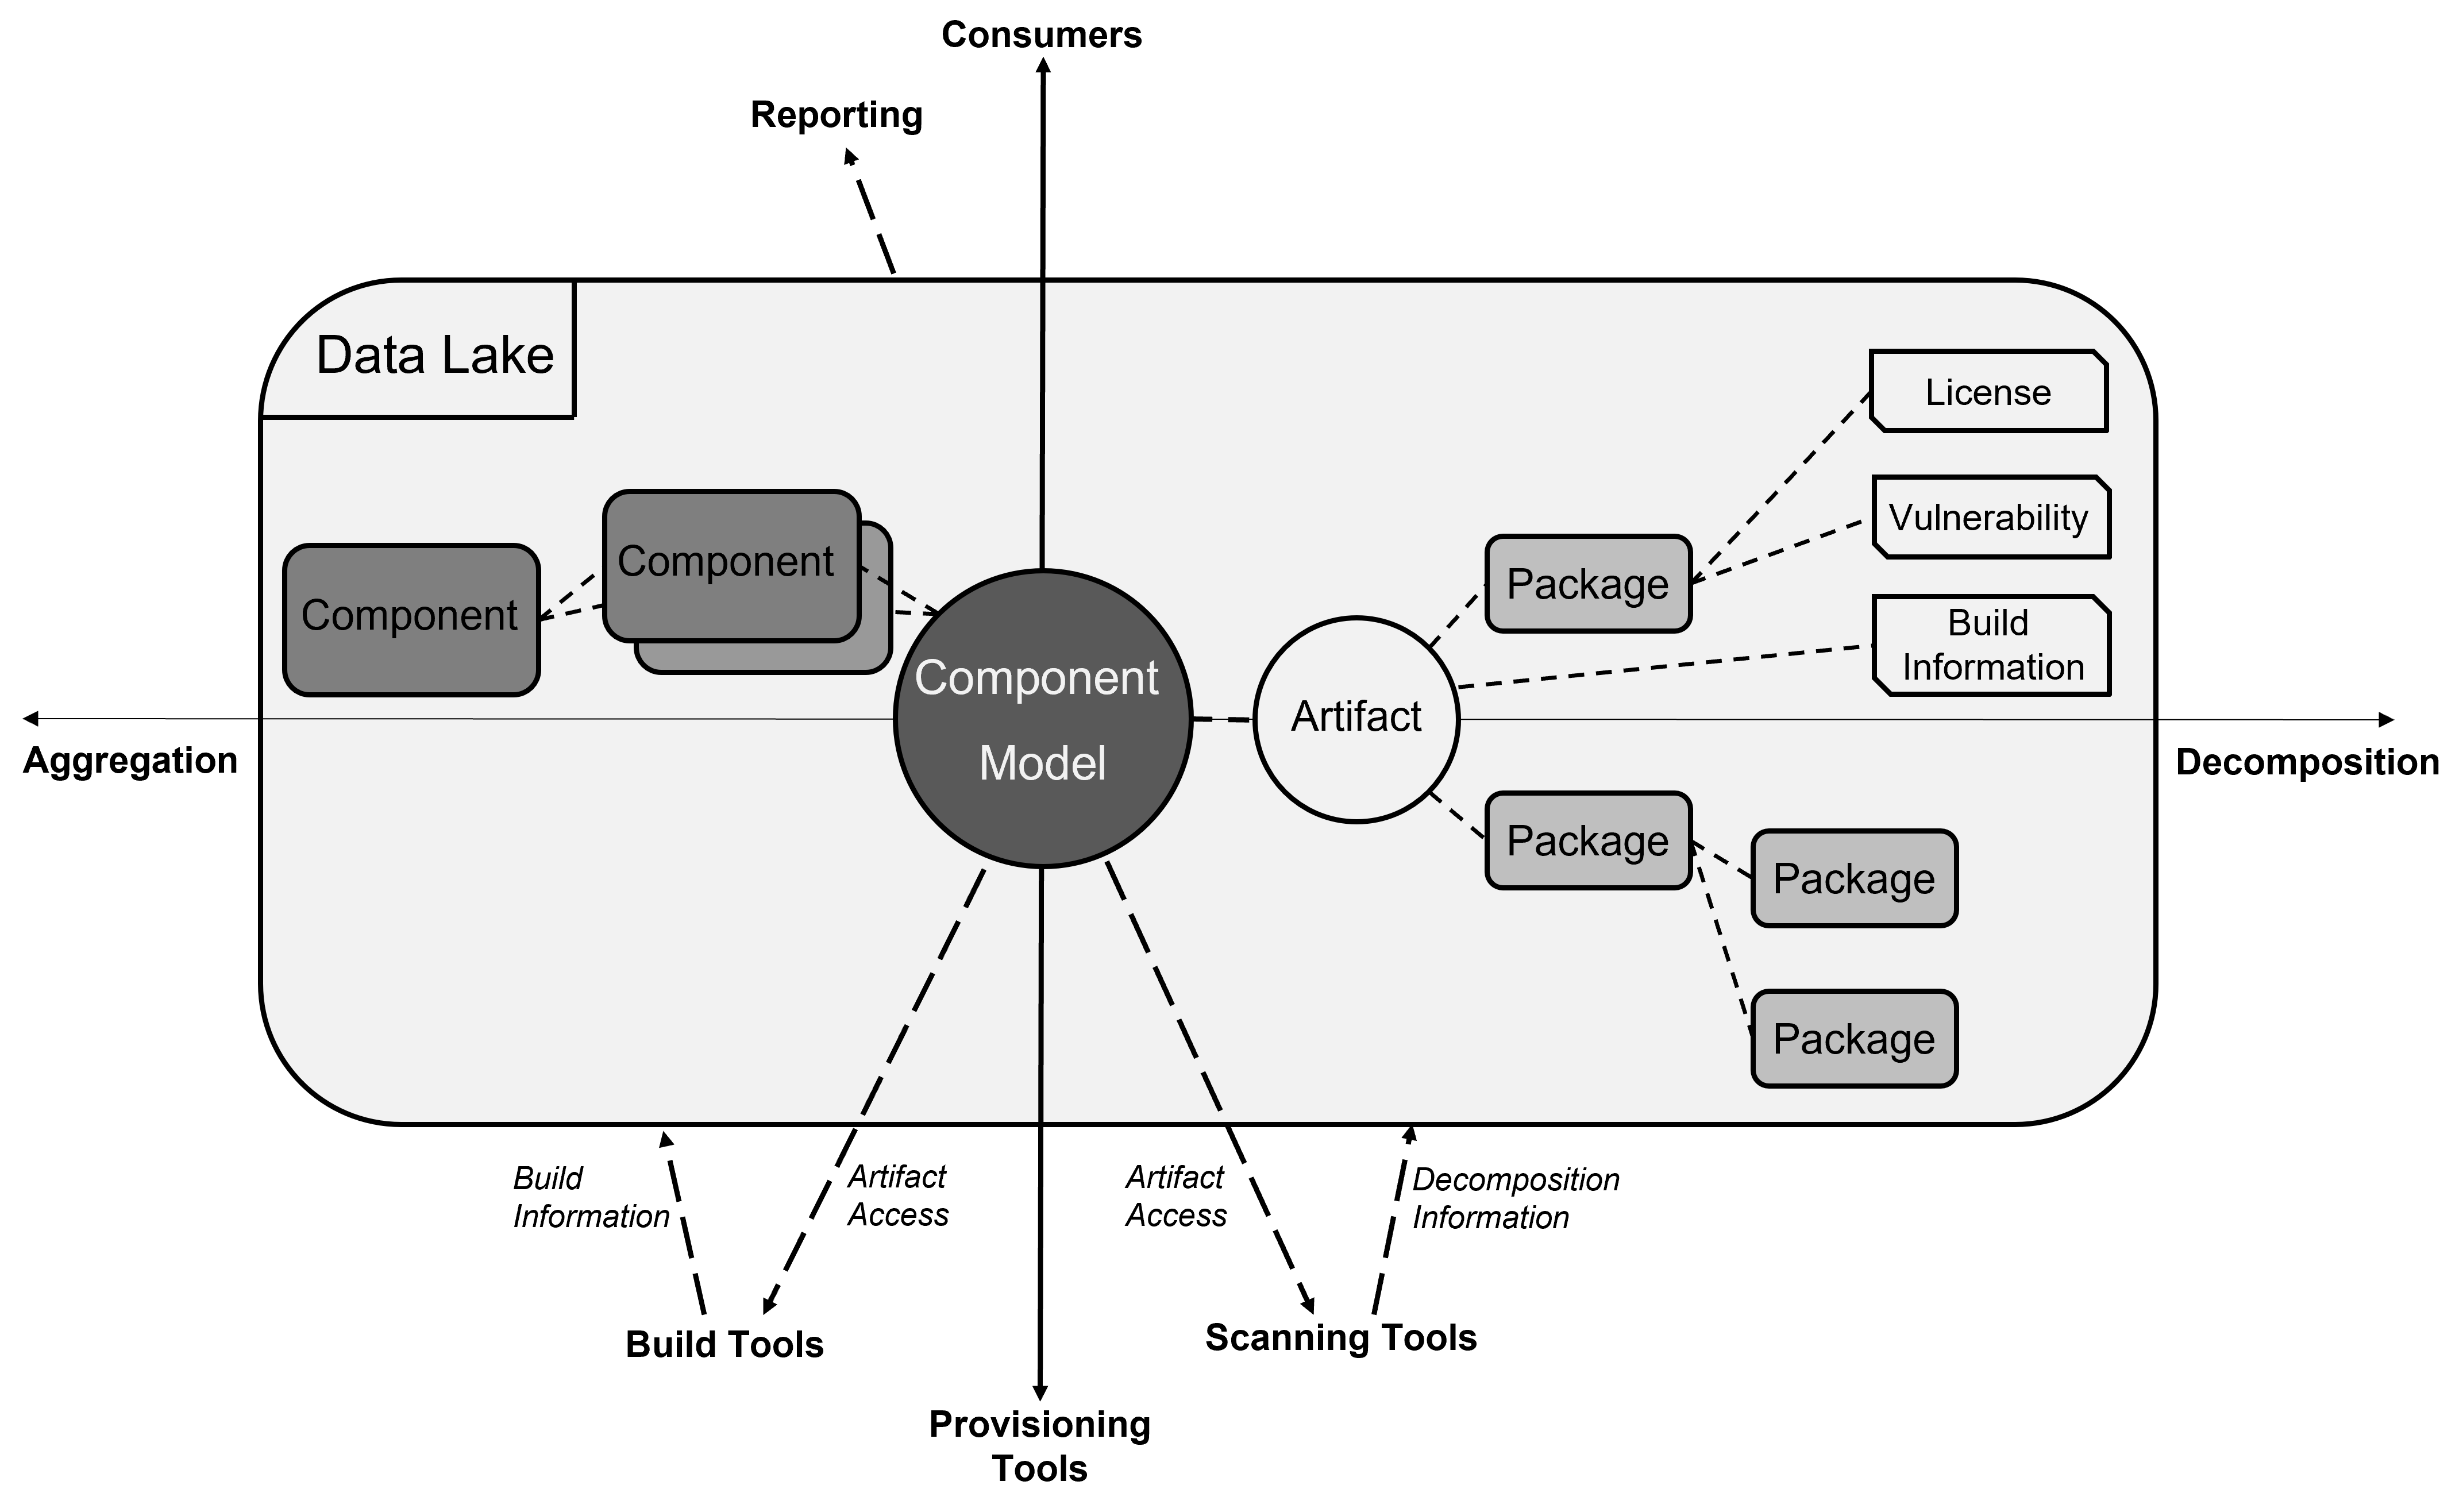
\includegraphics[scale=0.46]{abstract_datalake_design}
	\caption[Abstract Data Lake Design]{Abstract Data Lake Design \source{Own Representation}}
	\label{fig:AbstractDataLakeDesign}
\end{figure}


\subsection{Reference Integration Architecture} \label{sec:Reference Integration Architecture}
As already indicated in the previous chapters, although the \emph{Security and Compliance Data Lake} is an application for storing all kinds of metadata, the initial primary use case is storing the data resulting from scanning tools, thus dependencies, vulnerabilities and licenses. Below figure \ref{fig:DataLakeIntegration} shows the architecture designed for the integration into a modern development and deployment landscape based on the \emph{Open Component Model}.\par
The \emph{Data Collection Service} is the central component of this architecture. Its job is to orchestrate the process flow to derive metadata from information provided by the OCM and ingest it into the \emph{Data Lake}. In practice, this would be done based on policies, requiring to trigger the data collection once a day or based on some kind of event.\par 
In order to actually start the process, the Data Collection Service sends a request to the \emph{Access Service} (1). The Access Service is a transparency layer already built into the \emph{Component Repositories} as part of the OCM. Thus, if the Data Collection Service requests a set of Component Versions and their referenced Artifacts, the Access Service first fetches the corresponding Component Descriptors from the Component Repository (2). After receiving this information, the Access Service evaluates the access attribute in the referenced Sources and Resources and sends respective requests to the \emph{Source} and \emph{Resource Repositories} to fetch the Artifacts (3). Finally, the Access Service may return all the requested information to the Data Collection Service.\par

\begin{figure}[H]
	\centering
	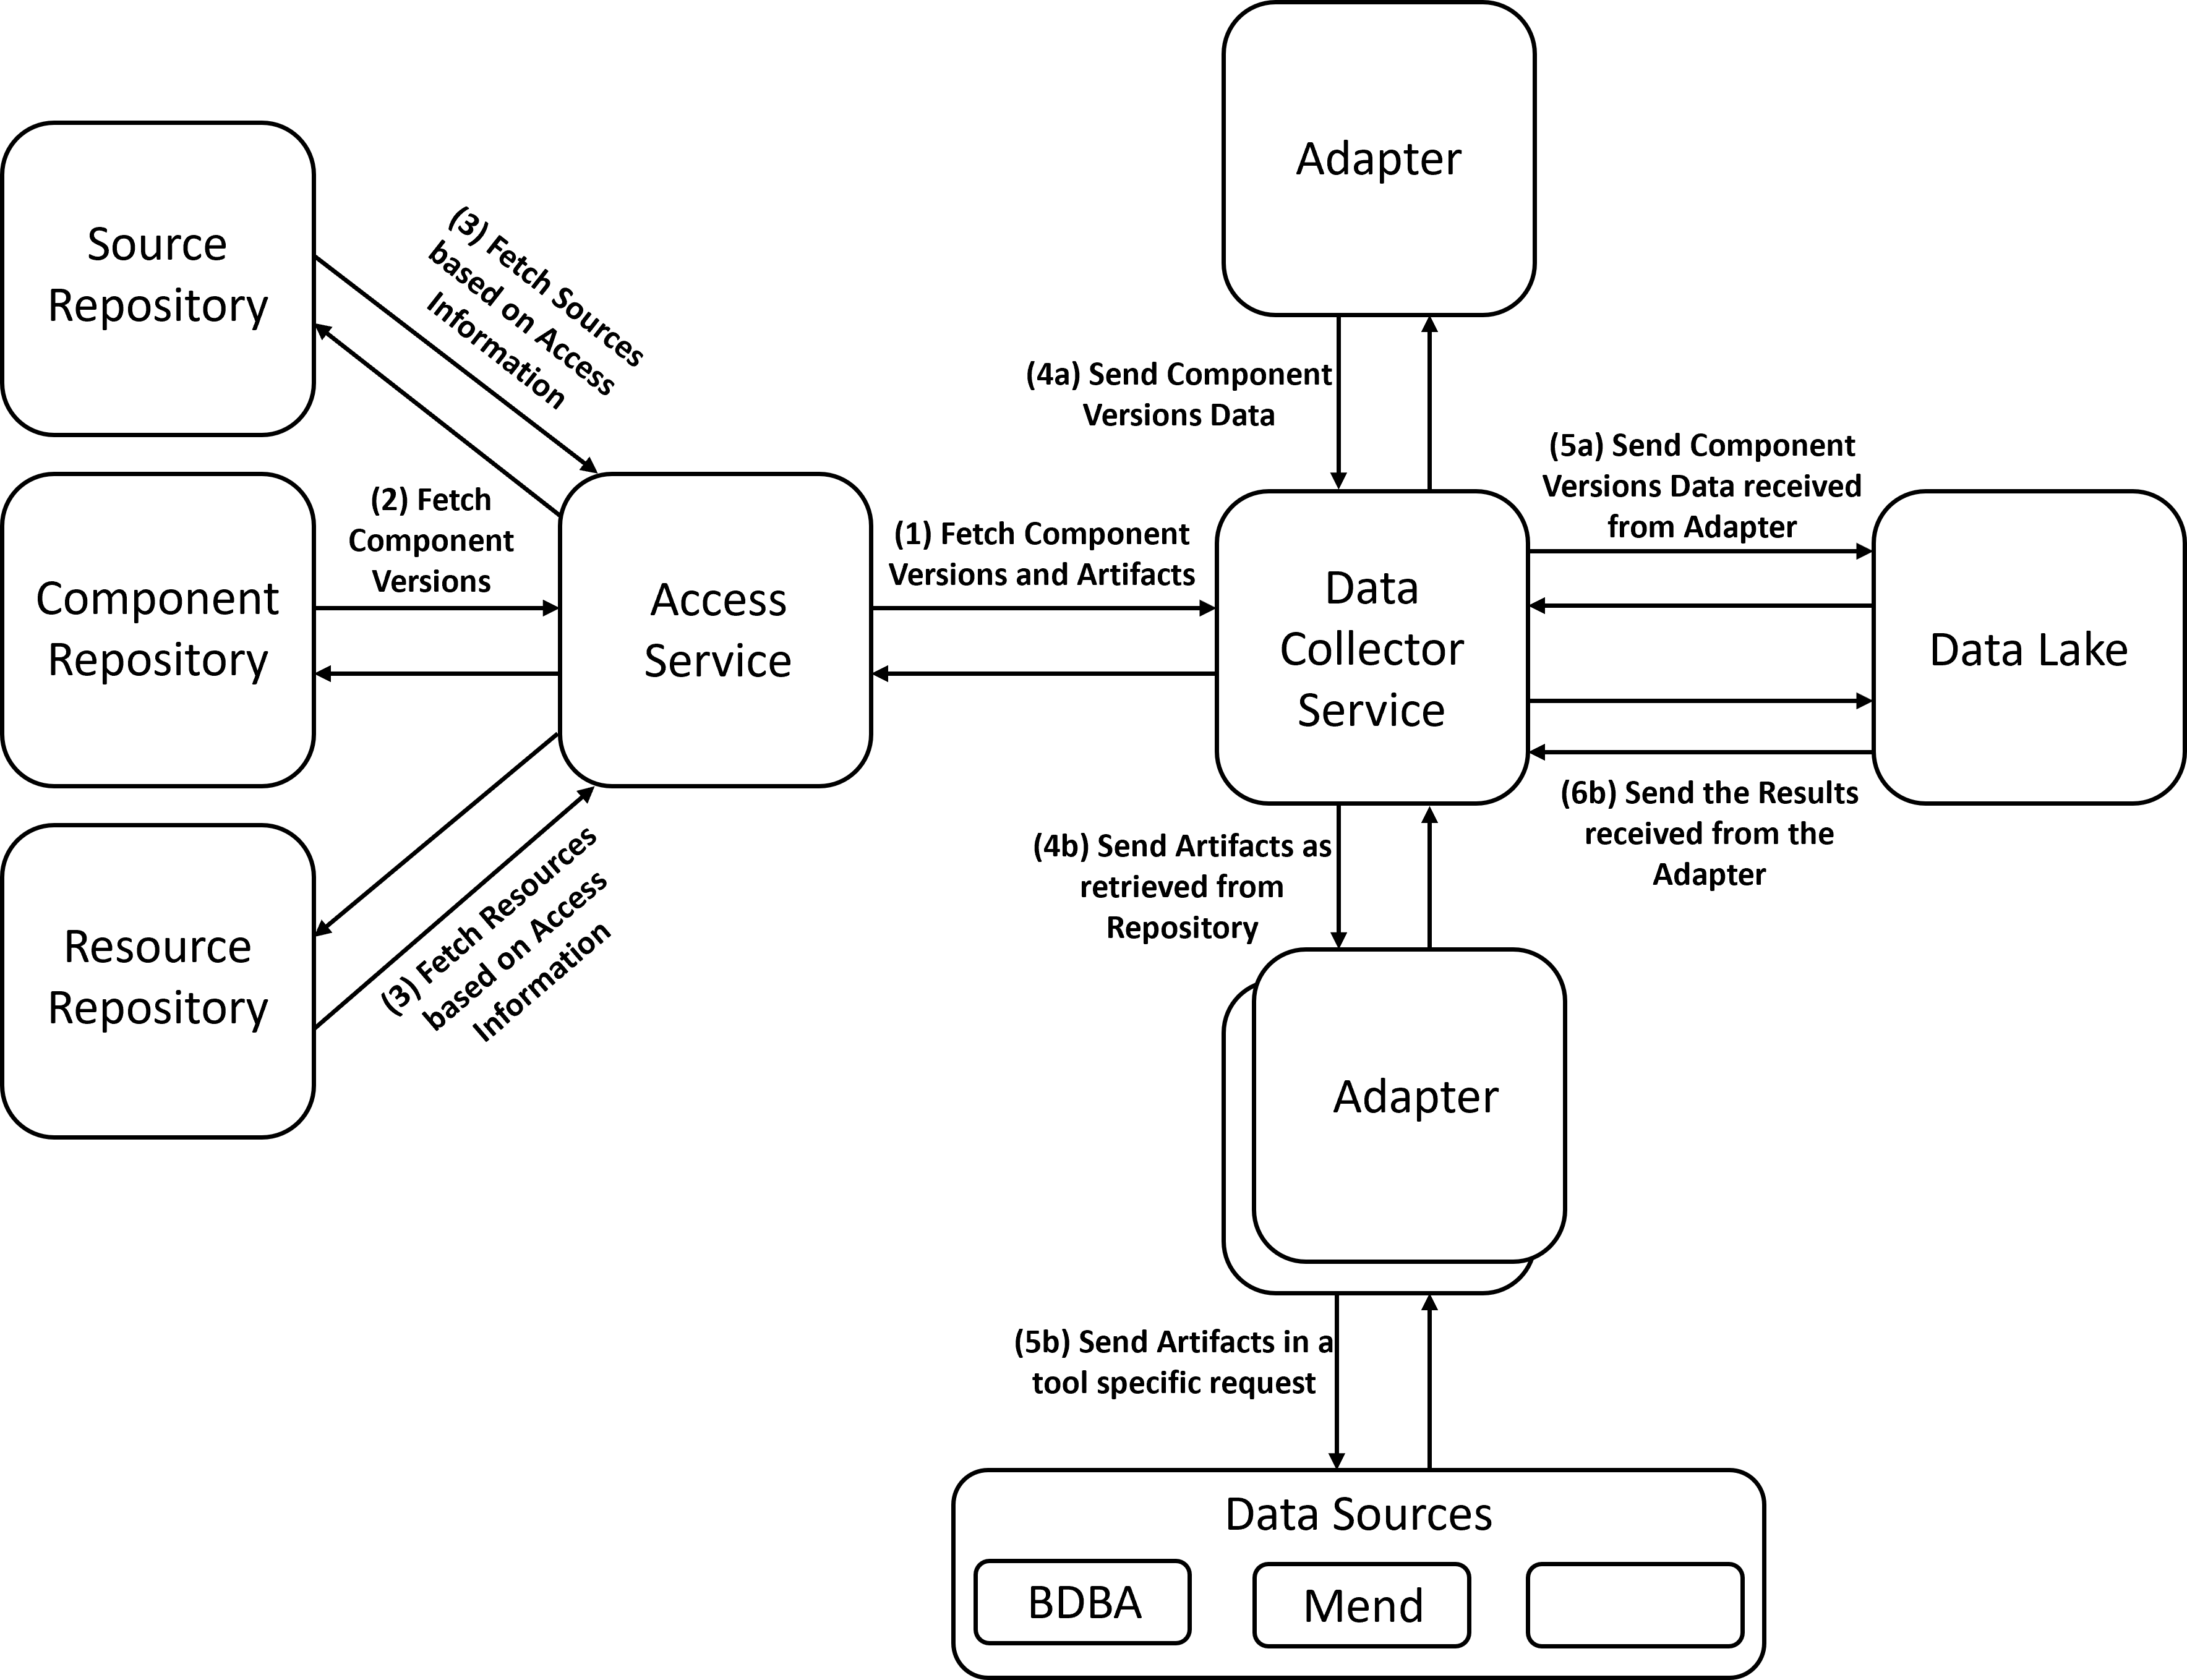
\includegraphics[scale=0.5]{datalake_integration}
	\caption[Data Lake Integration]{Data Lake Integration \source{Own Representation}}
	\label{fig:DataLakeIntegration}
\end{figure}

As shown in the figure, based on this information, there are two requests flows that may be triggered by the Data Collection Service, (4a) and (4b). The request flow illustrated above the Data Collection Service (4a) sends the Component Versions data, so the Component Descriptors, to an \emph{Adapter} which adjusts and returns this data in the format required for the consumption by the Data Lake.\par 
The request flow below the Data Collection Service (4b) distributes the Artifacts to a set of Adapters. Here, the Adapters initially wrap the Artifacts into the format required by a specific Data Source. In this case, there would be an Adapter for each scanning tool. Upon receipt of the scan results, these Adapters also adjust the data to the format required for consumption by the Data Lake, before returning it to the Data Collection Service.\par 
Finally, the Data Collection Service may send all the information, thus, the information acquired from the Component Versions about Components, Resources, Sources and their relationships (5a) as well as the information from the scanning tools about dependencies, vulnerabilities and licenses within these Artifacts (6b) to the Data Lake.\par
There were no communication protocols mentioned so far. This is due to the facts, that it does not really matter on the conceptual level and that the final implementation of this integration architecture is out of the scope of this thesis. But in practice, the communication between Data Collection Service and Access Service, between Adapters and Data Sources and between Data Collection Service and Data Lake will be over HTTP. The Adapters however will most likely not be implemented as discrete services but as components within Data Collection Service and therefore communicate over shared memory. Since it is very likely that additional Data Sources shall be added later on, the important part on the conceptual level is to still logically separate the components. Thus, there should be well defined interfaces between the Adapters and the Data Collection Service.\\

Some additional information about this integration architecture. Since the \emph{Component Model} enables automated access to all artifacts of any software product (or other kind of artifact aggregation), this integration architecture is completely decoupled from the rest of the development and deployment landscape. Thus, even in very complex development and deployment landscapes with several CI/CD pipelines based on different technologies (e.g. Jenkins or GitHub Actions) and including multiple different repositories, as long as it uses a \emph{Component Model}, this reference architecture does not have to be adjusted.\par
Even though the implementation of the integration architecture is out of scope of this thesis and is therefore not further discussed, it is still developed on a proof of concept basis as part of this work to feed actual real world data of the SAP Gardener into the \emph{Security and Compliance Data Lake}.

\subsection{Holistic Solution Architecture}
To conclude this chapter, this section provides a complete picture of a development and deployment landscape overcoming the limitations identified in the previous chapter for the state of the art approach through leveraging the \emph{Open Component Model} and the \emph{Security and Compliance Data Lake}.

\begin{figure}[H]
	\centering
	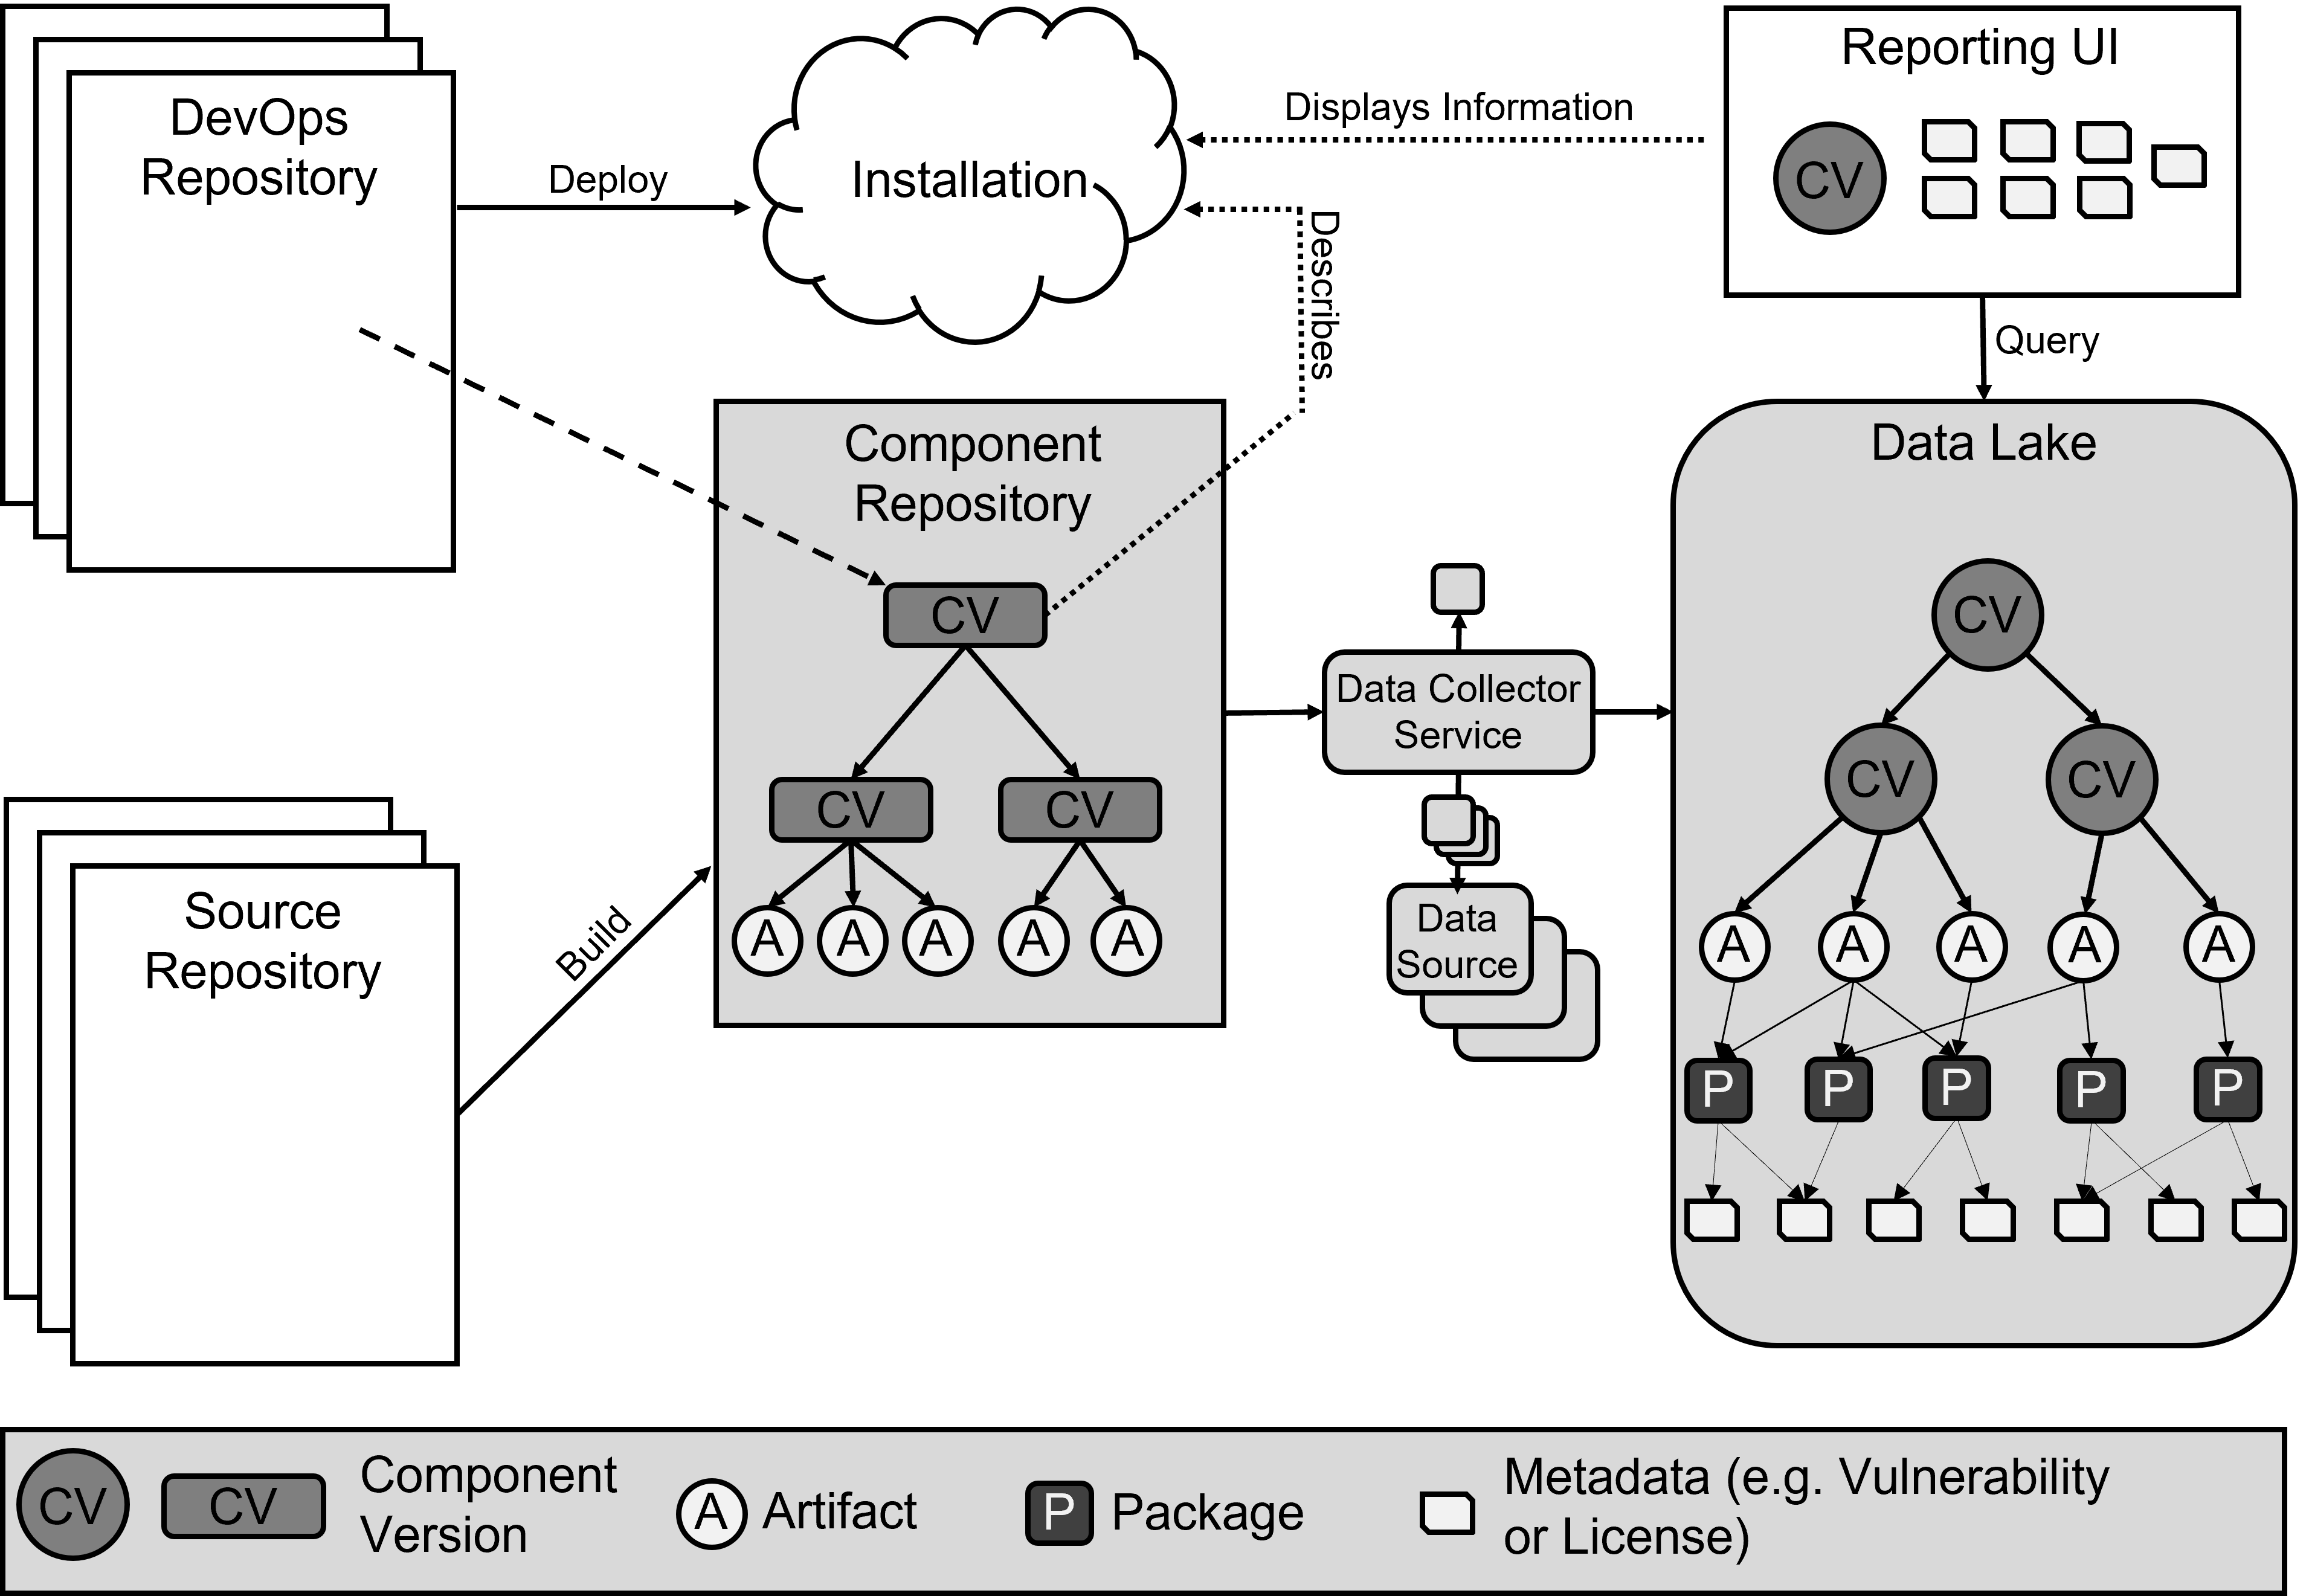
\includegraphics[scale=0.5]{holistic_solution_architecture}
	\caption[Holistic Solution Architecture]{Holistic Solution Architecture \source{Own Representation}}
	\label{fig:HolisticSolutionArchitecture}
\end{figure}

On the left side, figure \ref{fig:HolisticSolutionArchitecture} shows the whole process from build to deployment, or in other words from the \emph{Source Repository} over the \emph{Component Model Repository} and the \emph{DevOps Repository} to the \emph{Deployment} of a concrete software installation.\par
On the right, it shows the integration architecture from figure \ref{fig:DataLakeIntegration}. This visualizes the decoupling of the integration architecture previously mentioned. Everything is only linked through the \emph{Component Model}.\\

In a \emph{Build} process, \emph{Artifacts} may be build from \emph{Sources} stored in a \emph{Source Repository}. The \emph{Sources} also contain information to build a \emph{Component Version} describing the \emph{Sources} and \emph{Resources}.\par
Thereby, it is irrelevant where the technical artifacts are actually stored. They may be stored in the \emph{Component Repository} alongside the \emph{Component Versions} as indicated in the figure or they may be stored in specific artifact repositories. This information is provided by the \emph{Access Specification}. Through a built in \emph{Access Service}, as introduced in the previous section, the location of the artifacts is completely transparent to other tools accessing them through the \emph{Component Model}.\par
Consequently, the \emph{DevOps Repository} may merely contain a file specifying the \emph{Component Version} describing the software product version that shall be deployed to the \emph{Installation} environment. The rest may be automated with respective deployment tools.\par
The \emph{Data Lake} collects and combines metadata about the \emph{Component Versions} in the \emph{Component Model Repository} from different \emph{Data Sources} providing a consolidated view onto the complete set of software.\par
Thereon, a \emph{Reporting UI} may query information from the \emph{Data Lake} about the \emph{Component Version} describing a specific installation. So, an administrator or user may ask, which vulnerabilities and licenses are contained in this installation and the \emph{Data Lake} may conveniently traverse the relationships to retrieve this information. The development of a respective \emph{Reporting UI} is out of the scope of this thesis.\par
Ultimately, this holistic solution architecture enables \emph{answering} the question posed in section \ref{sec:Limitations} "Limitations" of the state of the art approach, about \emph{which product versions might be affected by a specific vulnerability}.\par
